\section*{Summary}

%Il Paper che si è deciso di analizzare è un documento risalente al 
%2016 che mostra lo sforzo di 6 ricercatori provenienti dall'Università 
%del Michigan e di Saarbrucken (Germania) . 
%Il documento mostra come l'utilizzo delle GAN (Generative Adversial Newtworks)
%permette un avanzamento nella generazione di immagini sintetiche partendo 
%da una descrizione testuale . 
%Esso mette a confronto il metodo proposto dalla ricerca e le 
%precedenti architetture che per quanto lontane dal traguardo descritto 
%sono in grado di ottenere rappresentazioni di feature testuali valide . 
%In particolare il paper vuole mostrare l'efficaccia del modello nel 
%generare immagini di uccelli e fiori partendo da una precisa descrizione 
%testuale degli stessi .
The paper that has been chosen for analysis is a document from 2016 
that showcases the effort of six researchers from the University of 
Michigan and Saarbrücken (Germany). 
The document shows how the use of GANs (Generative Adversarial Networks) 
allows for advancements in the generation of synthetic images starting 
from a textual description. 
It compares the method proposed by the research with previous architectures
that, although far from the described goal, are capable of obtaining 
valid textual feature representations. 
In particular, the paper aims to demonstrate the effectiveness of 
the model in generating images of birds and flowers based on a precise 
textual description of them.

\section*{Introduction}

In 2016, the ability of an AI system to generate realistic and 
coherent images from textual descriptions 
(such as "small red bird with a blue beak") was a current issue and 
far from being achieved.
It should be noted that it's necessary to use natural language 
and domain-specific attributes to describe the image to be generated.


 \subsection*{Related Papers \& Architectures}
 This paper is based on 3 documents that serve as a starting 
 point and tools for the proposed model:
 \begin{itemize}[noitemsep]
    \item \texttt{(Farhadi et al., 2009; Kumar et al., 2009;
    Parikh \& Grauman, 2011; Lampert et al., 2014)}: 
    3 Useful Papers for Encoding Distinctive Features of Objects 
    into Vectors (such as attributes used to distinguish 
    between different classes of objects)
    \item \texttt{(Fu et al., 2014 ; Akata et al., 2015)}: 
    2 Papers on "zero-shot" recognition, that is, recognizing 
    objects that have never been seen during the model's training.
    \item \texttt{(Yan et al., 2015).}: 
    And in Yan's paper, they discuss conditional image generation 
    in a manner similar to the method proposed here.
    \item \texttt{ (Reed et al., 2016)}: 
    Reed's paper presents highly discriminative and generic
    "zero-shot" text representations, 
    which are learnt automatically from words and characters.
    \item \texttt{(Goodfellow et al., 2014) \& (also studied
    by Mirza \& Osindero (2014) and Denton et al. (2015) )}: 
    Paper on application of conditional multi-modality for generative adversarial networks 

    \item \texttt{LEARNING A SHARED RAPPRESENTAZIONE ACROSS MODALITIES (MULTI-MODAL):}

    \item \texttt{Ngiam et al. (2011)}: 
    trained a stacked multimodal autoencoder on audio and video inputs and achieved a shared 
    modality-invariant representation.

    \item \texttt{Srivastava \& Salakhutdinov (2012)}: 
    developed a deep Boltzmann machine and jointly modeled images and text tags

    \item \texttt{Sohn et al. (2014) }
    proposed a multimodal conditional prediction framework

    \item \texttt{DEEP CONVOLUTIONAL DECODER NETWORK ARCHITECTURE :}
    
    \item \texttt{Dosovitskiy et al. (2015) \& Yang et al. (2015)}
    Used a deconvolutional network (with many layers of convolution and upsampling) 
    to create 3D chair representations based on shape, location, and illumination.
    And Yan added an encoder network to this approach .
    They trained a recurrent neural encoder-decoder to rotate 3D chair models
    and human faces based on rotational action sequences.

    \item \texttt{Reed et al. (2015)}
    Used a convolutional decoder to predict visual parallels between forms, video game characters, and 3D automobiles.

    \item \texttt{Goodfellow et al. (2014)}
    Introduced generative adversarial networks (GANs) and showed how GANs benefit from convolutional decoder networks for the generator module.

    \item \texttt{GENERATIVE ADVERSIAL NETWORK ....}
    
    \item \texttt{Denton et al. (2015)}
    Used a Laplacian pyramid of adversarial generators and discriminators to synthesize images 
    at multiple resolutions, producing high-resolution images and allowing generation conditioned on class labels

    \item \texttt{Radford et al. (2016)}
    Developed a stable and effective GAN architecture using a standard convolutional decoder, 
    incorporating batch normalization to improve image synthesis quality.

    \item \texttt{MULTI-MODAL LEARNING  }


    \item \texttt{Vinyals et al. (2015), Mao et al. (2015), Karpathy \& Li (2015), Donahue et al. (2015):}
    Introduced the use of recurrent neural network (RNN) decoders to generate text descriptions conditioned on images.

    \item \texttt{Hochreiter \& Schmidhuber (1997): }
    Used Long Short-Term Memory (LSTM) networks conditioned on top-layer features of deep convolutional networks 
    to generate image captions, especially with datasets like MS COCO.

    \item \texttt{Xu et al. (2015): }
    Incorporated a recurrent visual attention mechanism to further improve the results of text generation from images.

    \item \texttt{Ren et al. (2015) :}
    Generated replies to inquiries concerning picture visual content.

    \item \texttt{Wang et al. (2015) :}
    Expanded on Ren et al.'s technique by including an explicit knowledge foundation in the replying process.

    \item \texttt{Zhu et al. (2015) :}
    Used sequence models to align text (from books) and movies, allowing for simultaneous alignment of both.

    \item \texttt{Mansimov et al. (2016) :}
    Created pictures from text captions using a variational recurrent autoencoder with attention, 
    comparable to the DRAW model, which synthesized images in many stages.

    \item \texttt{Gregor et al. (2015) :}
    Created the DRAW model, which influenced Mansimov's way of producing graphics step by step.
    And obtaining realistic result also with "zero-shot" descriptions showing generalization . 

    \item \texttt{}
    \item \texttt{}


\end{itemize}

\section*{Datasets}
Bird and Flower images from human-written descriptions .

\begin{itemize}[noitemsep]
    \item \texttt{Caltech-UCSD Birds Database (Wah et al., 2011) ( CUB )} : 
    Dataset used in related Papers previously described and in this one as well .
    \item \texttt{Oxford-102 Flowers Dataset}
    Dataset used in this paper that correspond to have 5 text descriptions per image .
    \item \texttt{Test Dataset - MS COCO Dataset (Lin et al., 2014)}
    In addition to birds and flowers more general images and text descriptions .
\end{itemize}

\section*{How to reach the goal ?}
The difficulty of translating words into images may be 
divided into two subproblems.
\begin{itemize}[noitemsep]
    \item \texttt{1.} : 
    First, learn a feature vector from a specific text 
    based on the visualization we want to obtain .
    \item \texttt{2.} : 
    Given these features through the use of a certain architecture, 
    create a realistic and coherent image.
\end{itemize}

\subsection*{Effective Problems}
The paper highlights an intrinsic problem: when trying to generate images from textual descriptions, 
there are many different configurations that can be correct. ( Multi-modal Problem ). 
And even the reverse task, that is, generating descriptions from images, is difficult, 
but it is easier because it can be handled by predicting one word at a time, 
based on what has already been generated and the image itself.

\subsection*{Current Paper innovation ? }
Our technique differs from previous conditional GANs by focusing on text descriptions rather than class labels. 
This is the first design capable of differentiating from character to pixel level. 
The paper develop a manifold interpolation regularizer for the GAN generator, 
which enhances sample quality, including "zero-shot" categories on CUB.
It describes a model that generates 64x64 visually convincing pictures from text using a GAN. 
It differs from other models that just employ GANs for post-processing.
In practice it used a character-level text encoder and class-conditional GAN and 
focus in implementing a new architecture ad using it on fine-grained  
image datasets described before ( BUC and Oxford Flowers ) .
Testing on MOCO dataset and test set disjoint from Training set 
can return a strong indicator on the performance of the system .

\section*{Background knowledge}

\subsection*{
    GAN
}
The GAN architecture consist of two principal component :
Generator (G) and Discriminator (D) .
The main goal of D is to distinguish between real training images and generated images coming 
from G .
The idea is to maximize the logaritm of the loss of the Discriminator sampling images both from training set and 
generated while at the same time minimizing the outcoming of the log of 1 minus the loss of the Discriminator which has 
as input the generated image from random noise .

%  Log function 

\begin{figure}[h!]
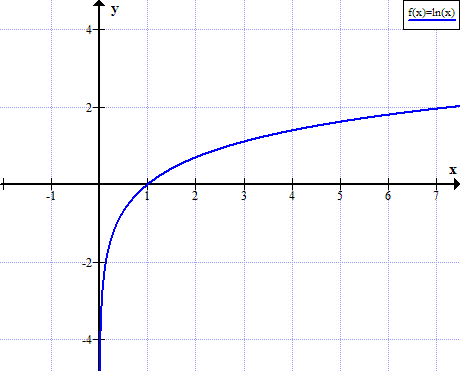
\includegraphics[width=80mm]{log.png}
\caption{Log Function}
\end{figure}
The Log function has a domain and an image that ranges from 0 to $\infty$.
It is possible to see that when the argument of the function tends to zero, the limit tends to -$\infty$, 
and when the argument tends to +$\infty$, the limit also tends to +$\infty$.

% Formula 
\subsection*{Formula}
\begin{equation}
    \min_{G} \max_{D} V(D, G) = \mathbb{E}_{x \sim p_{\text{data}}(x)}[\log D(x)] 
\end{equation}
\[
+ \mathbb{E}_{z \sim p_z(z)}[\log(1 - D(G(z)))]
\]
\begin{itemize}
    \item $D(x)$: the Discriminator as output layer use the Sigmoid function which map the data in a
    range from 0 to 1 .
    \item $G(x)$: the Generator instead as output layer use the Tanh function which map the data in a
    range from -$\infty$ to $\infty$ .
\end{itemize}

Therefore, based on these outputs and the behavior of the log function, it is possible to understand why 
the generator is minimized and the discriminator is maximized in the formula.
\\\\
So in detail the log function of the first expected value must have as arguments elements between 0 and 1 at most 
(output of D), therefore the first part of the equation, trying to maximize D, sees mainly negative values and at 
most equal to 0. \\
At the same time, the second equation with the second expected value calculates the difference between [ 1 - D(G(z)) ] 
, and since the argument of D tends to -infinity and we are simultaneously trying to maximize D and minimize G, 
the difference will result in a value between 0 and 1 (always positive).
Therefore, the limit of the logarithm as it approaches 0 will be equal to -$\infty$, 
while if the argument is 1, then the result is zero. \\
It's also possible to maximize G and use the log( [ D(G(z)) ] ) equation instead of log( [ 1 - D(G(z)) ] ) and 
obtain the same result . 


\subsection*{
    Text Encoder and Image Encoder via CLIP
}
To obtain a vector representation of text descriptions the main paper used the approch 
of Reed in 2006 using Deep convolutional and simmetric architecture based on both 
images a its corresponding text description . \\
The main idea in to have a dataset (Training set ) composed of N elements : 
\\
$ \{(v_n, t_n, y_n) : n = 1, ..., N\} $
\\
in which :
\begin{itemize}
    \item $ v_n $: correspond to the N images
    \item $ t_n $: correspond to the N text description
    \item $ y_n $: correspond to the class label ( usually there are more than two usually M )
\end{itemize}

First of all the paper define the classifier for both images and text description :
\begin{equation}
    f_v(v) = \arg \max_{y \in \mathcal{Y}} \mathbb{E}_{t \sim \mathcal{T}(y)} [\phi(v)^T \varphi(t)]
\end{equation}
    
\begin{equation}
    f_t(t) = \arg \max_{y \in \mathcal{Y}} \mathbb{E}_{v \sim \mathcal{V}(y)} [\phi(v)^T \varphi(t)]
\end{equation}

So in the first equation from all the possible class labels ($y$) we are trying to find the one that maximize the correlation between 
the input image and all the text descriptions on all the classes . \\
To do it we compute the multiplication between the encoded version of the input image $v$ and the current text description ($t$)
related to the current class . \\
In practice $\phi(v)$ and $\varphi(t )$ return a vector and we compute the similarity via a vector multiplication that return a scalar .\\ 
To compute the expected value in practice we compute the mean of all the scalar that we obtain from 
this multiplication on the specific class ($y$) .\\
In the second equation the formula is similar but on the input text description ($t$) .
The main idea was that an encoded description should have an higher compatibility 
with the images related to its class and so obtain higher value 

\begin{itemize}
    \item $\mathcal{Y}$: Set of the classes in which the images are divided .
    \item $\mathcal{T}(y)$: Set of the text description related to the $y$ class .
    \item $\mathcal{V}(y)$: Set of the images related to the $y$ class .
    \item $f_v(v)$: Classifier based on the images which return the class with higher compatibility with the image $v$
    \item $f_t(t)$: Classifier based on text description which return the class with higher compatibility with the description $t$
    \item $\phi(v)$: Image Encoder rappresentation on $v$ already trained on different dataset which return a vector (es. Obtained via CNN ).
    \item $\varphi(t)$: Text Encoder rappresentation on $t$ already trained on different dataset which return a vector (es. Obtained via CNN or LSTM).
    \item $\Delta$: Hinge or 0-1 loss for classification defined in which if the argument is higher than 0 it return 0 or 1 otherwise
    \item $\mathbb{E}_{t \sim \mathcal{T}(y)}$: Expected value in which $t$ correspond to all the text description related at the $y$ class .
    \item $\mathbb{E}_{v \sim \mathcal{V}(y)}$:  Expected value in which $v$ correspond to all the images related at the $y$ class .
\end{itemize}

Hinge or 0-1 Loss in this case is:

\begin{equation}
    \Delta( y, f(x) ) = max (0 , 1 - y * f(x) )
\end{equation}



\begin{equation}
    \varphi_{loss} = \frac{1}{N} \sum_{n=1}^{N} \Delta(y_n, f_v(v_n)) + \Delta(y_n, f_t(t_n)) 
\end{equation}

The main idea to compute the $\varphi_{loss}$ loss function was to learn the weights of 
the Text Encoder ($\varphi$) and fine-tuning it on our dataset .

During our implementation part this fine-tuning part has been done on 
the CLIP (Contrastive Language-Image Pre-Training) Text Encoder on the 
complete CUB and Flower dataset , in such a way to obtain 
relevant vector rappresentation which is composed of values that ranges 
from negative to positive values .

\section*{ Methodology }
All the methods are based on a GAN architecture with a Generator G 
and a Discriminator D . \\ 
And use ($\varphi$) as Text Encoder that is a character-level convolutional-
recurrent neural network .

The generator is defined as :
\[
G : \mathbb{R}^Z \times \mathbb{R}^{T} \rightarrow \mathbb{R}^D,
\]
And the discriminator is defined as :  
\[
D : \mathbb{R}^D \times \mathbb{R}^{T} \rightarrow \{0, 1\},
\]
where 
\begin{itemize}
    \item ${D}$: is the dimension of the generated image
    \item ${Z}$: is the dimension of the input noise 
    \item ${T}$: is the dimension of the text emdedded with $\varphi$
    \item ${D}$: is the dimension of the generated image
\end{itemize}

\subsection*{- Generator Part -}
First of all the generated image is defined as :
\[
\hat{x} \leftarrow G(z, \varphi(t))
\]
This Generator take as input a noise vector of dimension Z 
(In our implementation Z = 100) whose values are sampled from a Gaussian 
distribution between 0 and 1
\\
\[
z \in \mathbb{R}^Z \sim \mathcal{N}(0, 1)
\]
and the vector coming from the Text Encoder $\varphi$ for the specific 
text description t obtaining $\varphi(t)$ .
\\
First part - Projection \\
The first step of the Generator Net is to reduce the dimension of 
$\varphi(t)$ using one fully-connected layer to project 
to the dimension of the projection P . \\
This part continue using a Normalization Layer (BatchNorm1d)
and a Leaky-Relu as activation function with a specific negative slope .  
So the values on the vector can be negative and positive depending on the 
situation .

In our implementation $\varphi$ correspond to CLIP while \\
T is equal to 512 and \\
P is equal to 128 \\
After this first part an 128-dim vector is obtained and defined as :
\[
 p = projection( \varphi(t) )
\]

Second part - Concatanation \\
To compose the Latent Space vector (LSV) the paper suggested to concatenate 
the noise vector z with the projected vector p .

In our specific implementation the latent space has a dimension of H (H=228)
which is simple the concatation of the two vector of dimension T=100 
and P=128 .

\[
h = concat( z , p )
\]

Third part - Final Net to generated the image 64x64 RGB 
As input of the Final Net part of the Generator is the Latent Space Vector 
(LSV) of dimension H (H=228). 

This Final Net is composed of 4 set of layers in which the first one is a 
Convolutional Transpose 2D Layers ( "to up-sample" ) followed by a Normalization layer 
and Relu as activation function so we only have values greater than 0 .

In our implementation the initial dimension of the vector was (228,1,1) but 
after only the first Convolutional Transpose layer it is projected into an higher dimension of 
(512,8,8) .

After using the other 3 set of layers the dimension will be equal to (64,32,32) .
The last layer is useful because permit to obtain an image of the shape 
(3,64,64) and is composed of a Convolutional Transpose 2D Layer and Tanh as activation function .

Using Tanh with in input values coming from the last layer that can be positive and 
negative as well due to the weight of the 2D Convolutional Transpose Layer we will obtain an 
image 64x64 with 3 channel RGB with values that ranges from -1 to 1 due to Tanh .
\[
\hat{x} = generate( h )
\]
And G is defined as this 3 Parts applied in order one after another  . 


\subsection*{- Discriminator Part -}
The Discriminator is defined as this :
\[
D ( \hat{x} , \varphi(t) ) = \left\{ x_i \in [0, 1] \mid i = 0, 1, \dots, 120 \right\}
\]
It takes in input the generated image $\hat{x}$ and depending
on the situation an encoded version of the text description $\varphi(t)$
related or not to image generated .

Similarly to what we have seen in the Generator Part the Discriminator is 
sub-divided in 3 Parts or Networks . 

First Net - Down-Sampling 
The First Part is composed of a several (in our implementation 4) set 
of Convolutional 2D Layers ("to down-sample") 
followed by a normalization Layer (BatchNorm2d except the first set)
and Leaky-Relu as activation function . 
After passing through this Net the generated image of a shape of (3,224,244)
will have a dimension of (512,14,14) .
\[
 q = DownSampling( \hat{x} )
\]

Second Part - Projection Text Emdedding and Concatenation

This part consist of two phases and it take as argument the down-sampled generated 
image ${q}$ and the encoded version of the text description $\varphi(t)$ .
The first phase consist in projecting $\varphi(t)$
in a lower-dimension P (P=128) using one fully-connected layer and normalization layer 
followed by a Leaky-Relu as activation function in the exact same way that we have done in 
the Generator .
After this first phase a 128-dim vector is obtained and defined as :
\[
 p = projection( \varphi(t) )
\]
The last task of the first phase was to adapt the project dimension of p 
( that is (128,1,1) ) in such a way to be compatibile with the second phase 
which concatenate p with q . 
So the dimension of p is squeezed into a dimension that allow to concatenate
the two data and it became (128,14,14)
\[
 \hat{p} = squeeze( p )
\]

The second Phase consist of the concatenation of $q$ and $\hat{p}$ 
which result in a dimension of (512+128, 14, 14) = (256, 640, 14, 14)
This concatation permit to obtain the Latent vector c :
\[
 c = concatenate( q , \hat{p} )
\]


Third Part - Final Net 
This Final Net it's only composed of One Convolutional 2D Layer and 
Sigmoid as activation function which map the input in a range that goes 
from 0 to 1 .
The first Convolution Layer modify the shape from (256, 640, 14, 14) 
to (512,4,4) while the sigmoid function change its shape into
( 1,11,11 ) .
At the end of this phase we flatten the 11x11 values into a vector of 
121-dimension .
So at the end for each generated image and text Emdedding we obtain a 
121-dim vector rappresenting the discriminator factors .
\[
 d\_loss = FinalNet( c )
\]

--------------------------

\subsection*{(Vanilla GAN) :  Generative Adversarial Network without Conditional Latent Space }
The Vanilla implementation stands for an implementation in which the Generator only depend 
on the noise vector z and not depend on the Conditional Latent Space $ \varphi(t) $ and the same 
stand for the discriminator which depends only on the actual or the generated image .

\subsection*{(GAN-CLS) :  Generative Adversarial Network with Conditional Latent Space }
The idea behind this architecture is to use $\varphi$ as Text Encoder (CLIP)
to create the embeddings related to text description ${t}$ coeherent with the image (${x}$) 
to obtain ${h}$ and one not correlated to the image sampled randomly $\hat{t}$ to obtain $\hat{h}$ .
Another step is to generate the Noise Vector ${z}$ randomly sampled from a Gaussian 
Distribution . \\
The following step is to generate an image passing through ${z}$ and ${h}$ as explained 
in the Generator Part and otbaining $\hat{x}$ .
As well the Discriminator have to compute a value ${s_r}$ that correspond to 
the loss passing through it the real image ${z}$ and the corresponding text 
emdedding ${h}$ . \\
In the same way we obtain ${s_r}$ passing at inference time 
the image ${x}$ and $\hat{t}$ and we calculate 
${s_f}$ passing the image ${x}$ and ${h}$ . 
The Final part consist in computing the Discriminator loss $L_D$ as the 
$\log(s_r) + \left(\log(1 - s_w) + \log(1 - s_f)\right) / 2$ . \\
In the actual implementation the loss of the Discriminator is computed 
using the BCELoss (Binary Cross Entroy Loss) between ${s_r}$ and a 
"smoothed" version of the label filled with 1 computing "${d\_loss\_r}$" and again two times , first 
with ${s_f}$ and a "fake label" filled with 0 computing "${d\_loss\_f}$" and after using 
${s_f}$ and the "fake label" computing "${d\_loss\_f}$" . \\
So the final value is computed summing the 3 obtained values :
\[
 L_D = d\_loss\_f + d\_loss\_w + d\_loss\_r
\]
After this computation the Discriminator is updated using backpropagtion 
based on the gradient with $\alpha$ as parameter .

For the Generator Loss $L_D$ we don't compute only the logarithm
of ${s_f}$ (\ in Algorithm 1 )\ but we use a custom loss composed of 3 part .
The first one compute the BCELoss between ${s_f}$ and the "real label" which is
a vector filled with 1 . \\
The second one compute the MSELoss (\ Mean Squared Error Loss )\ between 
${q_r}$ (after Down-Sampling) and ${q_f}$ coming from the Discriminator of
${s_r}$ and ${s_f}$ . \\
The Third part is computed the L1Loss between the generated image $\hat{x}$
and the real image ${x}$ .
The 3 part are summed to obtain $L_G$
\[
 L_G = BCELoss( s_f,real\_label ) + MSELoss( q_r , q_f ) 
\]
\[
 + L1Loss(\hat{x},x)
\]
And finally after this computation the Generator is updated using backpropagtion 
based on the gradient with $\alpha$ as parameter .



\begin{algorithm}
    \caption{GAN-CLS training algorithm with step size $\alpha$, using minibatch SGD for simplicity.}
    \begin{algorithmic}
        \Require minibatch images $x$, minibatch matching text $t$, minibatch mis-matching text $\tilde{t}$, 
        number of training batches $S$
        \For{$n = 1$ to $S$}
            \State $h \leftarrow \varphi(t)$ \hfill \{Encode matching description\}
            \State $\hat{h} \leftarrow \varphi(\tilde{t})$ \hfill \{Encode mis-matching description\}\
            \State $z \sim \mathcal{N}(0, 1)^Z$ \hfill \{Extract Noise Vector\}
            \State $\hat{x} \leftarrow G(z, h)$ \hfill \{Forward through generator\}
            \State $s_r \leftarrow D(x, h)$ \hfill \{Real image, right text\}
            \State $s_w \leftarrow D(x, \hat{h})$ \hfill \{Real image, wrong text\}
            \State $s_f \leftarrow D(\hat{x}, h)$ \hfill \{Fake image, right text\}
            \State $L_D \leftarrow \log(s_r) + \left(\log(1 - s_w) + \log(1 - s_f)\right) / 2$
            \State $D \leftarrow D - \alpha \nabla L_D$ \hfill \{Update discriminator\}
            \State $L_G \leftarrow \log(s_f)$
            \State $G \leftarrow G - \alpha \nabla L_G$ \hfill \{Update generator\}
        \EndFor
    \end{algorithmic}
\end{algorithm}


\subsection*{(GAN-INT) :  Generative Adversarial Network Interpolated}
The main difference with respect with the previous implementation relies 
in the fact that Generation of the "fake image" do not depend not anymore 
only on z and t ,but in an interpolation of two different text emdeddings .
In practice the paper found that fixing ${\beta}$ = 0.5 works well and want to
underline that t1 and t2 may come from different images and 
even different categories.
This parte has not been implemented and tasted but with little modification
on the actual code can be performed . 


\begin{equation}
    \mathbb{E}_{h1,h2 \sim p_{data} } [\log( 1 - D(G( z , \beta h1 + 
    (1-\beta) h2 )))]
\end{equation}

\subsection*{- WGAN : - Wessertstain GAN}
This typology of GAN is not present in the Paper but follow the same concept 
described before . 
In principle we can observe first all the algorithm :

\begin{algorithm}
    \caption{WGAN training algorithm with step size $\alpha$, using minibatch SGD for simplicity.}
    \begin{algorithmic}
        \Require minibatch images $x$, minibatch matching text $t$, minibatch mis-matching text $\tilde{t}$, 
        number of training batches $S$ , number of iteraton for the Discriminator $NI$ 
        \For{$n = 1$ to $S$}
            \State $h \leftarrow \varphi(t)$ \hfill \{Encode matching description\}
            
            \For{$n = 1$ to $NI$}
                \State $z \sim \mathcal{N}(0, 1)^Z$ \hfill \{Extract Noise Vector\}
                \State $\hat{x} \leftarrow G(z, h)$ \hfill \{Forward through generator\}
                \State $s_r \leftarrow D(x, h)$ \hfill \{Real image, right text\}
                \State $s_f \leftarrow D(\hat{x}, h)$ \hfill \{Fake image, right text\}
                \State $L_D \leftarrow (s_r) - (s_f) $
                \State Clip weights of $D$ within $[-c, c]$
                \State \{Lipschitz constraint\}
            \EndFor
            \State $z \sim \mathcal{N}(0, 1)^Z$ \hfill \{Extract again Noise Vector\}
            \State $\hat{x} \leftarrow G(z, h)$ \hfill \{Forward through generator\}
            \State $s_f \leftarrow D(\hat{x}, h)$ \hfill \{Fake image, right text\}
            \State $L_G \leftarrow -(s_f) $ \hfill \{Wasserstein loss for Generator\}
            \EndFor
    \end{algorithmic}
\end{algorithm}

The idea behind this architecture is to use $\varphi$ as a Text Encoder to create embeddings 
related to a text description $t$ that matches the image $x$, obtaining $h$. 
This embedding $h$ serves as the condition for both the Generator and Discriminator. \\
Another step involves sampling a Noise Vector $z$ randomly from 
a Gaussian Distribution $\mathcal{N}(0, 1)^Z$. \\
The following step is to generate a fake image $\hat{x}$ by passing $z$ 
and $h$ through the Generator $G$. \\
The Discriminator $D$ computes a score $s_r$ by passing the real image $x$ and 
the corresponding text embedding $h$, which reflects how well $D$ recognizes 
the real data. \\
Similarly, the Discriminator computes a score $s_f$ by passing 
the generated image $\hat{x}$ and the same text embedding $h$.\\
The Discriminator loss $L_D$ is calculated as the difference $s_r - s_f$, which represents 
the Wasserstein distance. To enforce the Lipschitz constraint, the weights of 
the Discriminator are clipped within a fixed range $[-c, c]$ after every update. \\
This ensures the Discriminator satisfies the required gradient properties for stable training.
After training the Discriminator for multiple steps, the Generator is trained. \\
A new Noise Vector $z$ is sampled from $\mathcal{N}(0, 1)^Z$, and a fake image $\hat{x}$ 
is generated by passing $z$ and $h$ through $G$. \\
The Discriminator then computes a new score $s_f$ for this generated image, 
and the Generator loss $L_G$ is calculated as $-s_f$. \\
This encourages the Generator to produce images that maximize the Discriminator's score, 
effectively improving the quality of the generated images. \\
The training process alternates between optimizing the Discriminator and the Generator. 
Over multiple iterations, the Discriminator learns to distinguish real and fake images better, 
while the Generator learns to produce more realistic images. \\
This iterative process ensures that the Wasserstein distance between the real and generated 
data distributions is minimized, leading to stable and efficient GAN training.



